\documentclass[letterpaper]{article} % DO NOT CHANGE THIS
\usepackage[submission]{aaai2027}  % DO NOT CHANGE THIS (anonymous, double-blind)
% The serif, sans-serif, and monospaced fonts are loaded automatically by
% aaai2027.sty (newtxtext, helvet, courier). DO NOT add any font package.
\usepackage[hyphens]{url}  % DO NOT CHANGE THIS
\usepackage{graphicx} % DO NOT CHANGE THIS
\urlstyle{rm} % DO NOT CHANGE THIS
\def\UrlFont{\rm}  % DO NOT CHANGE THIS
\usepackage{natbib}  % DO NOT CHANGE THIS AND DO NOT ADD ANY OPTIONS TO IT
\usepackage{caption} % DO NOT CHANGE THIS AND DO NOT ADD ANY OPTIONS TO IT
\frenchspacing  % DO NOT CHANGE THIS
\usepackage{booktabs}
\usepackage{amsmath}
\usepackage{amssymb}
\pdfinfo{
/TemplateVersion (2027.1)
}

\setcounter{secnumdepth}{2}
\hyphenation{DENSEWORLD}

% AAAI-27 Bridge "Modeling and Simulating Human Behavior in the Age of AI: From Cognition to
% Society" (Cog2Soc). Rules (cog2soc.github.io, read 2026-11-26): research findings, experience
% reports, methods, theory, datasets, evaluation tools, demos, position papers; at most 4 pages
% EXCLUDING references, AAAI two-column format; anonymized for double-blind review; at least two
% reviews on relevance, substance, suitability for discussion; non-archival; OpenReview
% AAAI.org/2027/Bridge/Cog2Soc. The call asks each paper to explain the human phenomenon, the
% approach or research question, and the connection to another participating community.
% Deadline Nov 29 2026 23:59 AoE (= Nov 30 03:59 PST); notification Dec 10 2026 AoE.
% Dual submission is not stated: this work is also an AAAI-27 student abstract (non-archival)
% and is under review at Human-Centric AgMS; disclose both on OpenReview.
% Same paper as ../v1_Human_Centric (title, data, numbers); only the framing differs, plus the
% student-abstract review fix W2: no "data effect" claim (full fine-tuning was not run at 115k).
% Anonymity: no author names, no links that identify the authors (GitHub and the project
% page are left out; the Hugging Face organisation is anonymous), own prior work not cited.
% Facts follow the code, not earlier drafts: factor targets come from Grounding DINO + SAM 3
% (src/m10_sam_segment.py); Causal L1 predicts the 2nd temporal half from the 1st
% (src/utils/pt_causal.py); the split is clip-level (src/utils/clip_splits.py); Ours is ONE
% fixed arm, surgical_3stage_DI_diheavy_encoder, in every cell of Table 1.

\title{FactorJEPA on DENSEWORLD-115k: Can a World Model Predict Crowded, Chaotic South Asian Streets?}

\author{Anonymous Submission}
\affiliations{}

\begin{document}

\maketitle

\begin{abstract}
On a crowded South Asian street, pedestrians, two-wheelers, auto-rickshaws, carts, and animals share one right of way and coordinate by negotiation rather than lane rules, often while partly hidden from each other. Models of such collective behaviour are often calibrated on sparser, lane-structured, mostly Western scenes, and so are video world models such as V-JEPA 2.1, which learn to forecast scenes from raw video in embedding space. We build DENSEWORLD-115k, 115,687 clips (276 hours) cut from 714 public YouTube videos of 22 Indian cities, released as metadata only, and FactorJEPA, which replaces V-JEPA's monolithic predictor with separate layout, agent, and interaction channels. Compared with seven adaptation methods under identical data and budgets, one fixed FactorJEPA configuration predicts masked and future content better at both 2B and 1B scale, and after full 115k-clip training it separates from the strongest rival on all four diagnostics of predictive structure by 13.9 to 43.3 widths of the paired 95\% confidence interval. Competing methods stay ahead on temporal coherence. We discuss what a world model learned from street video can and cannot yet offer the modelling and cross-cultural evaluation of collective behaviour.
\end{abstract}

\begin{links}
    \link{Dataset}{https://huggingface.co/datasets/anonymousML123/denseworld-115k}
\end{links}

\section{Introduction}

\paragraph{The human phenomenon.} On South Asian streets, road edges are negotiated rather than painted, pedestrians and vehicles of very different speeds share one right of way, clutter keeps road users partly hidden, and who goes first is settled by local norms more than by lane rules. Behaviour models from transport research and computational social science, such as social-force and agent-based models \cite{helbing1995social}, describe this coordination with hand-set interaction rules that must be calibrated on observed data, which often comes from sparser, lane-structured scenes. Large driving datasets such as BDD100K \cite{yu2020bdd100k} and nuScenes \cite{caesar2020nuscenes} sample this regime rarely.

\paragraph{Our approach.} We ask whether a world model can learn this collective behaviour directly from video. Joint Embedding Predictive Architectures (JEPA) such as V-JEPA 2.1 \cite{murlabadia2026vjepa21} learn without labels by predicting masked or future video content as embeddings rather than pixels. Their predictor is monolithic: nothing in it keeps the road layout, the individual road users, and the interactions between them apart inside the predicted future, so it cannot be read as a description of who yields to whom. We contribute:
\begin{itemize}
    \item \textbf{DENSEWORLD-115k}, a 276-hour drive-through, walk-through, and aerial video corpus of 22 Indian cities, released as reconstructible metadata.
    \item \textbf{FactorJEPA}, a V-JEPA predictor that composes the future from layout, agent, and interaction channels, with no extra inputs at inference.
    \item A controlled comparison against seven adaptation methods at two model scales and two data scales, reporting one fixed configuration on 13 diagnostics, including those it loses.
\end{itemize}
\paragraph{Connection across communities.} The agent and interaction channels give machine learning a structure that behavioural science already uses (individuals and their pairwise couplings), and give behaviour modellers a cross-cultural corpus and a learned predictor to compare their rules against.

\begin{figure*}[t]
\centering
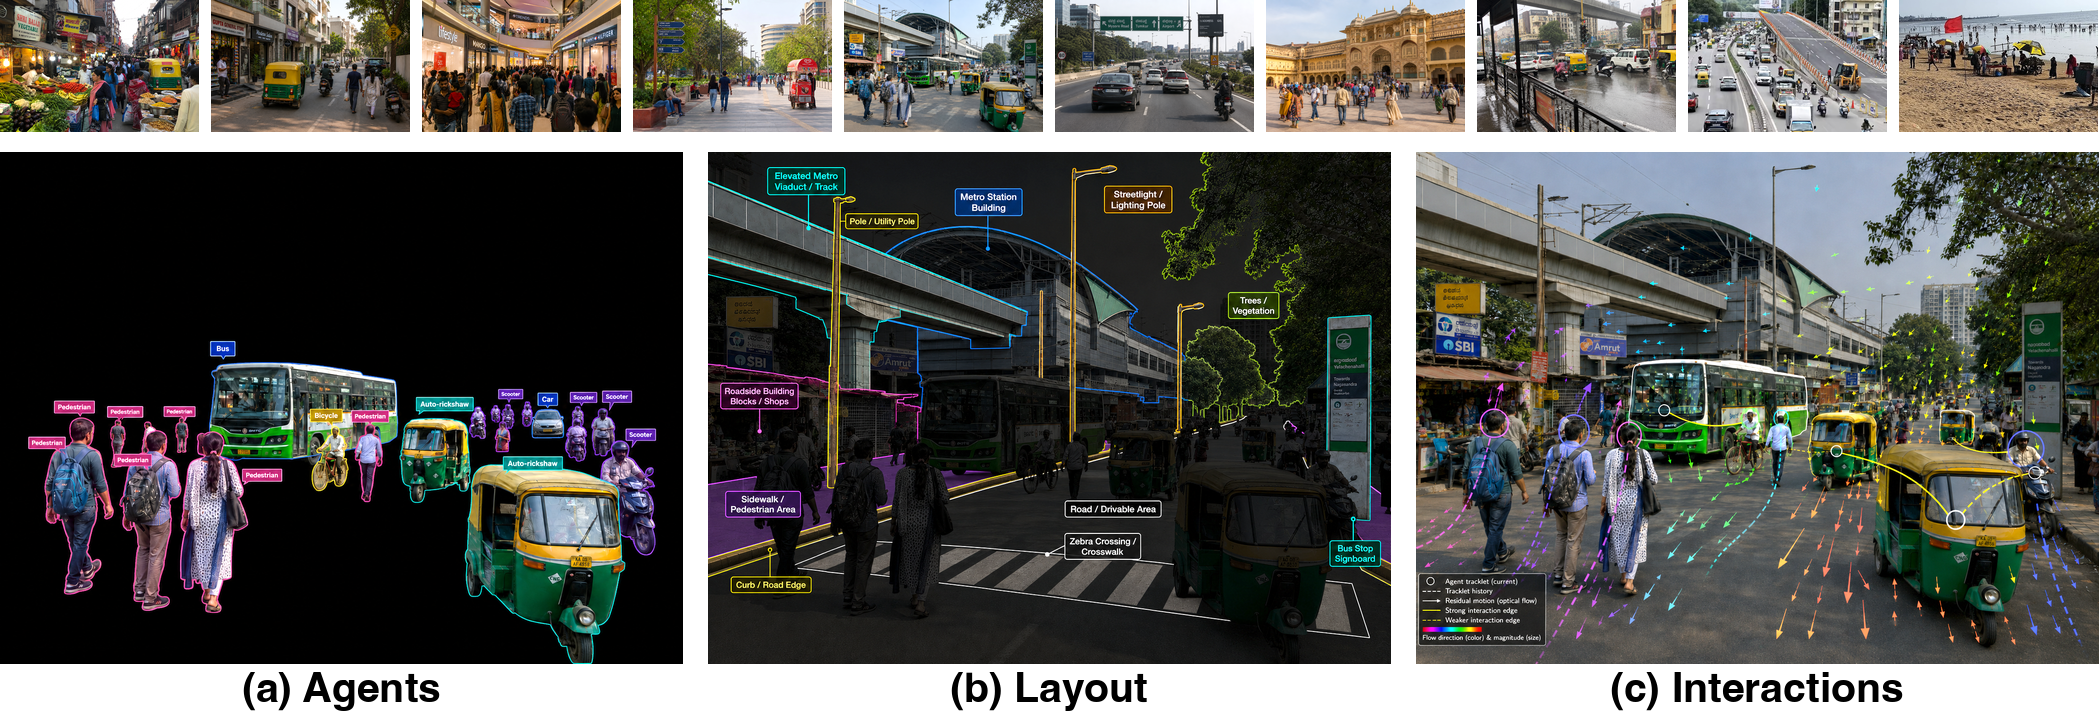
\includegraphics[width=\textwidth]{figures/denseworld_teaser.png}
\caption{DENSEWORLD-115k. Top: ten scene types, left to right: market, residential, commercial, promenade, transit, highway, heritage, junction, flyover, and beach. Bottom: one scene factorized into (a) agents, (b) layout with agents suppressed, and (c) interactions: circles mark tracked agents, arrows encode motion (colour: direction; length: magnitude), and solid or dashed edges mark stronger or weaker coupling.}
\label{fig:teaser}
\end{figure*}

\section{DENSEWORLD-115k}

The corpus cuts 714 public long-form YouTube videos (480p) from 22 Tier-1 and Tier-2 Indian cities into 115,687 clips of 4 to 10 seconds with scene and shot-boundary detection, 276 hours in total (Figure~\ref{fig:teaser}, top). It covers drive-through, walk-through, and aerial viewpoints across markets, residential lanes, transit corridors, junctions, flyovers, heritage sites, and beaches, at different times of day and in different weather. Faces and licence plates are blurred before any processing. For 86,831 clips, an automatic pipeline derives layout, agent, and interaction targets: Grounding DINO \cite{liu2024groundingdino} detects agents on anchor frames, SAM~3 \cite{carion2025sam3} tracks their masks through the clip, and agent pairs are linked by proximity and relative motion.

Against a reference set of BDD100K and nuScenes clips grouped by the same scene types, DENSEWORLD has more agents per clip and a larger share of pixels covered by agents on all six types we compared (Figure~\ref{fig:density}); we measured only these two axes, not occlusion or interaction pressure. This is a cross-cultural gap in the data itself: a behaviour model calibrated on the Western reference would meet denser scenes here on every scene type.

\paragraph{Release.} The videos stay under their creators' copyright and are not redistributed. The dataset card ships the source list, the clip manifest with timestamps, and a deterministic script that rebuilds every clip from YouTube.

\begin{figure*}[t]
\centering
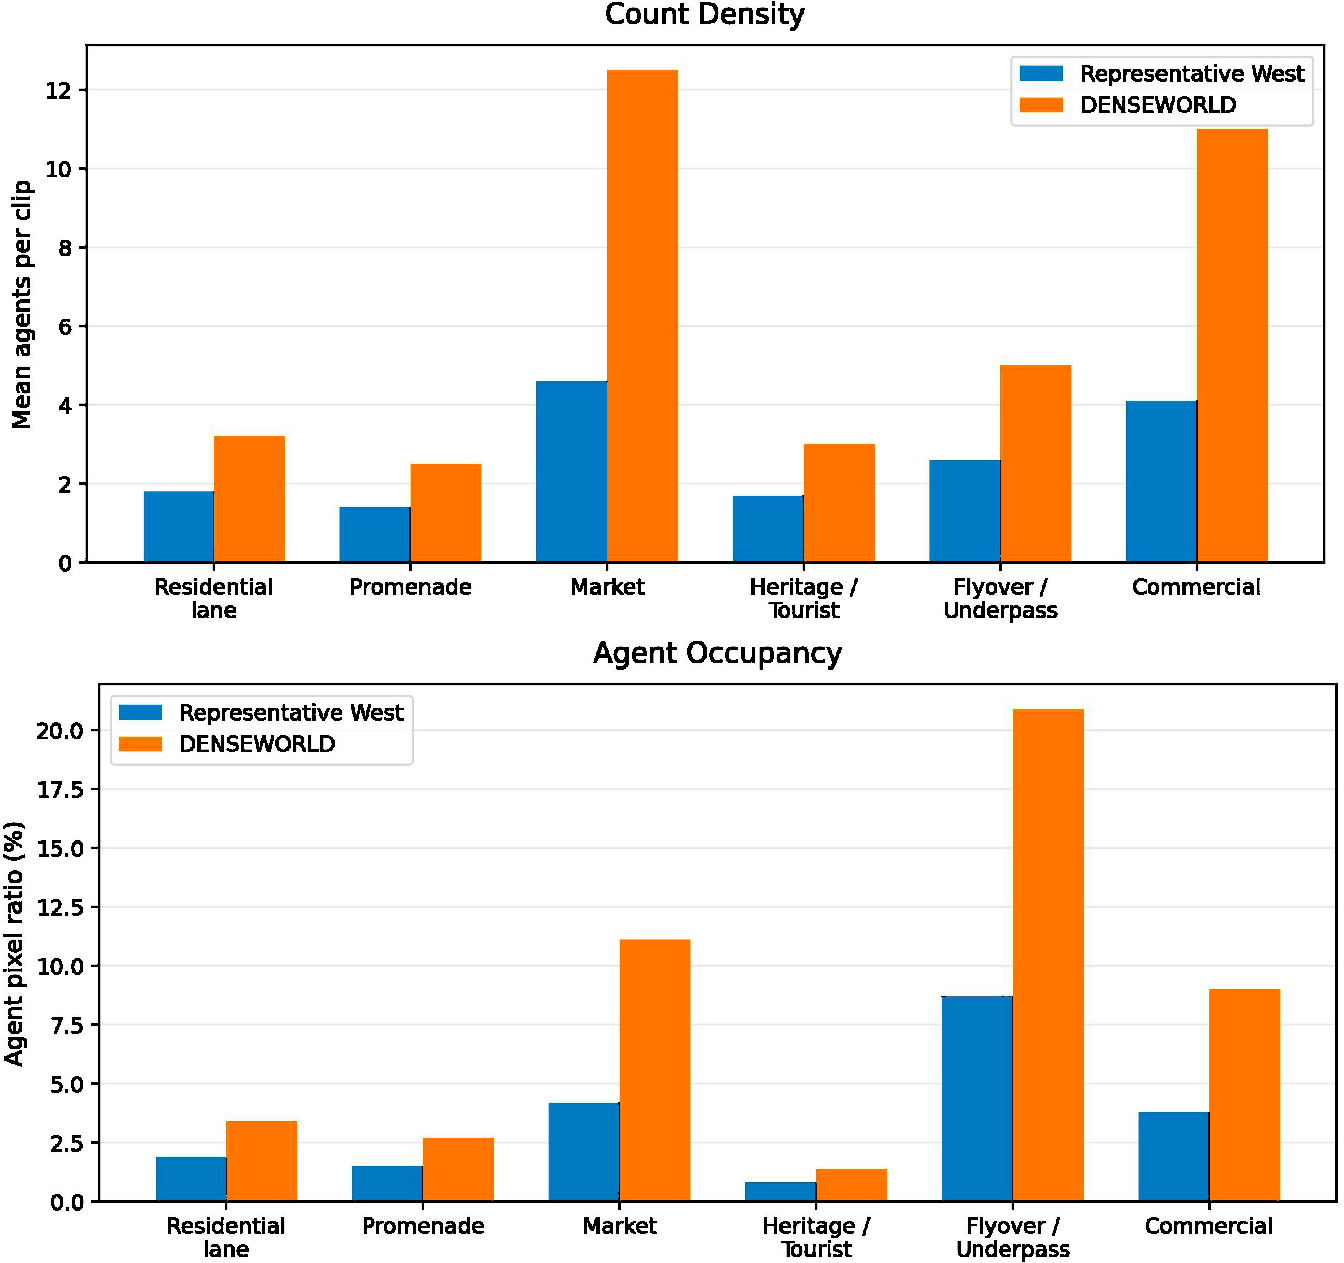
\includegraphics[width=0.85\textwidth]{figures/denseworld_vs_west_density_bold.pdf}
\caption{Mean agents per clip (top) and share of pixels covered by agents (bottom) for DENSEWORLD and a Western reference drawn from BDD100K and nuScenes, per scene type.}
\label{fig:density}
\end{figure*}

\section{FactorJEPA}

FactorJEPA keeps the V-JEPA 2.1 encoder, its momentum target encoder, the masking policy, and the prediction targets, and replaces only the predictor. For each target token it predicts layout, agent, and interaction coordinates $C_L$, $C_A$, $C_I$ (Figure~\ref{fig:teaser}, bottom) and composes the future embedding through learned dictionaries,
\begin{equation}
\widehat Y = C_L A_L^{\top} + C_A A_A^{\top} + C_I A_I^{\top}.
\end{equation}
A soft visibility gate re-weights agents by how visible they are instead of discarding occluded ones, and interaction coordinates are sparse weighted sums over candidate agent pairs. During training, the factor heads are anchored to the automatic layout, agent, visibility, and interaction targets of the training split, and a penalty on cross-channel covariance and kernel alignment limits shortcut mixing between channels. At inference the predictor reads only the encoder's context tokens: no detector, tracker, or agent proposal is needed, so the model runs wherever V-JEPA runs. Only the predictor and the top encoder blocks are trained. Unlike SlotFormer's object-centric slots \cite{wu2023slotformer} and DriveWorld's split of static scene from dynamics \cite{min2024driveworld}, FactorJEPA factorizes inside the JEPA embedding space and gives interactions their own supervised channel.

\section{Evaluation}

\paragraph{Protocol.}
We adapt V-JEPA 2.1 at 2B and 1B parameters on a stratified 10k-clip set, and the 1B model also on the full corpus. FactorJEPA is compared with the frozen backbone, full fine-tuning, linear probing then fine-tuning, continual self-supervised learning, LoRA \cite{hu2022lora}, DoRA \cite{liu2024dora}, and Auto-RGN \cite{lee2023surgical}, all under identical clips, masking, optimization steps, and splits. Test clips are held out at the clip level (1,825 in the 10k regime, 23,106 in the full regime); clips cut from the same source video can fall on both sides. Every margin is a paired 95\% BCa bootstrap interval over test clips.

\paragraph{Diagnostics of predictive structure.}
\emph{Future-frame L1}: error between predicted and target-encoder embeddings on the token blocks hidden by V-JEPA's mask generator. \emph{Causal L1}: the same error when the second half of a clip is predicted from its first half. \emph{Mask-ratio slope}: growth of that error as the hidden fraction rises from 0.3 to 0.9. \emph{Motion cosine}: how well a linear probe recovers clip motion from the embedding. Nine further diagnostics probe temporal coherence and semantics (Table~\ref{tab:headline}).

\begin{table}[t]
\centering
\small
\setlength{\tabcolsep}{2pt}
\begin{tabular}{lrrrrrr}
\toprule
 & \multicolumn{2}{c}{2B$\cdot$10k} & \multicolumn{2}{c}{1B$\cdot$10k} & \multicolumn{2}{c}{1B$\cdot$115k} \\
\cmidrule(lr){2-3}\cmidrule(lr){4-5}\cmidrule(lr){6-7}
Diagnostic & Ours & Rival & Ours & Rival & Ours & Rival \\
\midrule
future-frame L1 ($\downarrow$) & \textbf{0.496} & 0.504\textsuperscript{L} & \textbf{0.590} & 0.596\textsuperscript{L} & \textbf{0.573} & 0.589\textsuperscript{L} \\
causal-block L1 ($\downarrow$) & \textbf{0.529} & 0.533\textsuperscript{L} & \textbf{0.614} & 0.617\textsuperscript{L} & \textbf{0.597} & 0.607\textsuperscript{L} \\
mask-ratio slope ($\downarrow$) & \textbf{0.053} & 0.054\textsuperscript{L} & \textbf{0.052} & 0.053\textsuperscript{D} & \textbf{0.047} & 0.058\textsuperscript{L} \\
motion-cos ($\uparrow$) & 0.116 & \textbf{0.244}\textsuperscript{F} & 0.048 & \textbf{0.090}\textsuperscript{F} & \textbf{0.097} & 0.078\textsuperscript{L} \\
\midrule
temporal-order ($\uparrow$) & 0.944 & \textbf{0.947}\textsuperscript{Z} & 0.925 & \textbf{0.927}\textsuperscript{C} & \textbf{0.918} & 0.915\textsuperscript{Z} \\
pace ($\uparrow$) & 0.719 & \textbf{0.724}\textsuperscript{L} & 0.711 & \textbf{0.729}\textsuperscript{Z} & 0.703 & 0.703\textsuperscript{L} \\
action top-1 ($\uparrow$) & 0.500 & \textbf{0.528}\textsuperscript{C} & 0.483 & \textbf{0.509}\textsuperscript{F} & 0.567 & \textbf{0.572}\textsuperscript{L} \\
arrow-of-time ($\uparrow$) & 0.935 & \textbf{0.965}\textsuperscript{Z} & 0.957 & \textbf{0.965}\textsuperscript{Z} & 0.955 & \textbf{0.975}\textsuperscript{Z} \\
TCC $\tau$ ($\uparrow$) & 0.274 & \textbf{0.292}\textsuperscript{Z} & 0.287 & \textbf{0.334}\textsuperscript{Z} & 0.380 & \textbf{0.400}\textsuperscript{Z} \\
exposure-bias ($\downarrow$) & 0.048 & \textbf{0.038}\textsuperscript{C} & \textbf{0.034} & 0.036\textsuperscript{D} & 0.038 & \textbf{0.035}\textsuperscript{L} \\
rollout drift ($\downarrow$) & 0.011 & \textbf{0.008}\textsuperscript{C} & 0.005 & 0.005\textsuperscript{D} & 0.007 & \textbf{0.006}\textsuperscript{L} \\
L1-vs-$\Delta t$ ($\downarrow$) & 0.008 & \textbf{0.006}\textsuperscript{C} & 0.009 & \textbf{0.007}\textsuperscript{Z} & 0.009 & \textbf{0.007}\textsuperscript{Z} \\
TCC cycle ($\downarrow$) & 2.249 & \textbf{2.111}\textsuperscript{Z} & 2.416 & \textbf{2.195}\textsuperscript{Z} & 2.806 & \textbf{2.132}\textsuperscript{Z} \\
\bottomrule
\end{tabular}
\par\smallskip
{\small\raggedright
Rival superscript: L LoRA, D DoRA, F full fine-tuning, C continual self-supervised learning, Z frozen backbone. At 115k only LoRA and the frozen backbone were trained as rivals.\par}
\caption{One fixed FactorJEPA model (Ours, identical in every cell) against its strongest rival on 13 diagnostics. Above the rule: the four diagnostics of predictive structure; below: the rest, where the rival leads on most rows. Bold: the better of each pair (neither when equal).}
\label{tab:headline}
\end{table}

\begin{figure}[!tb]
\centering
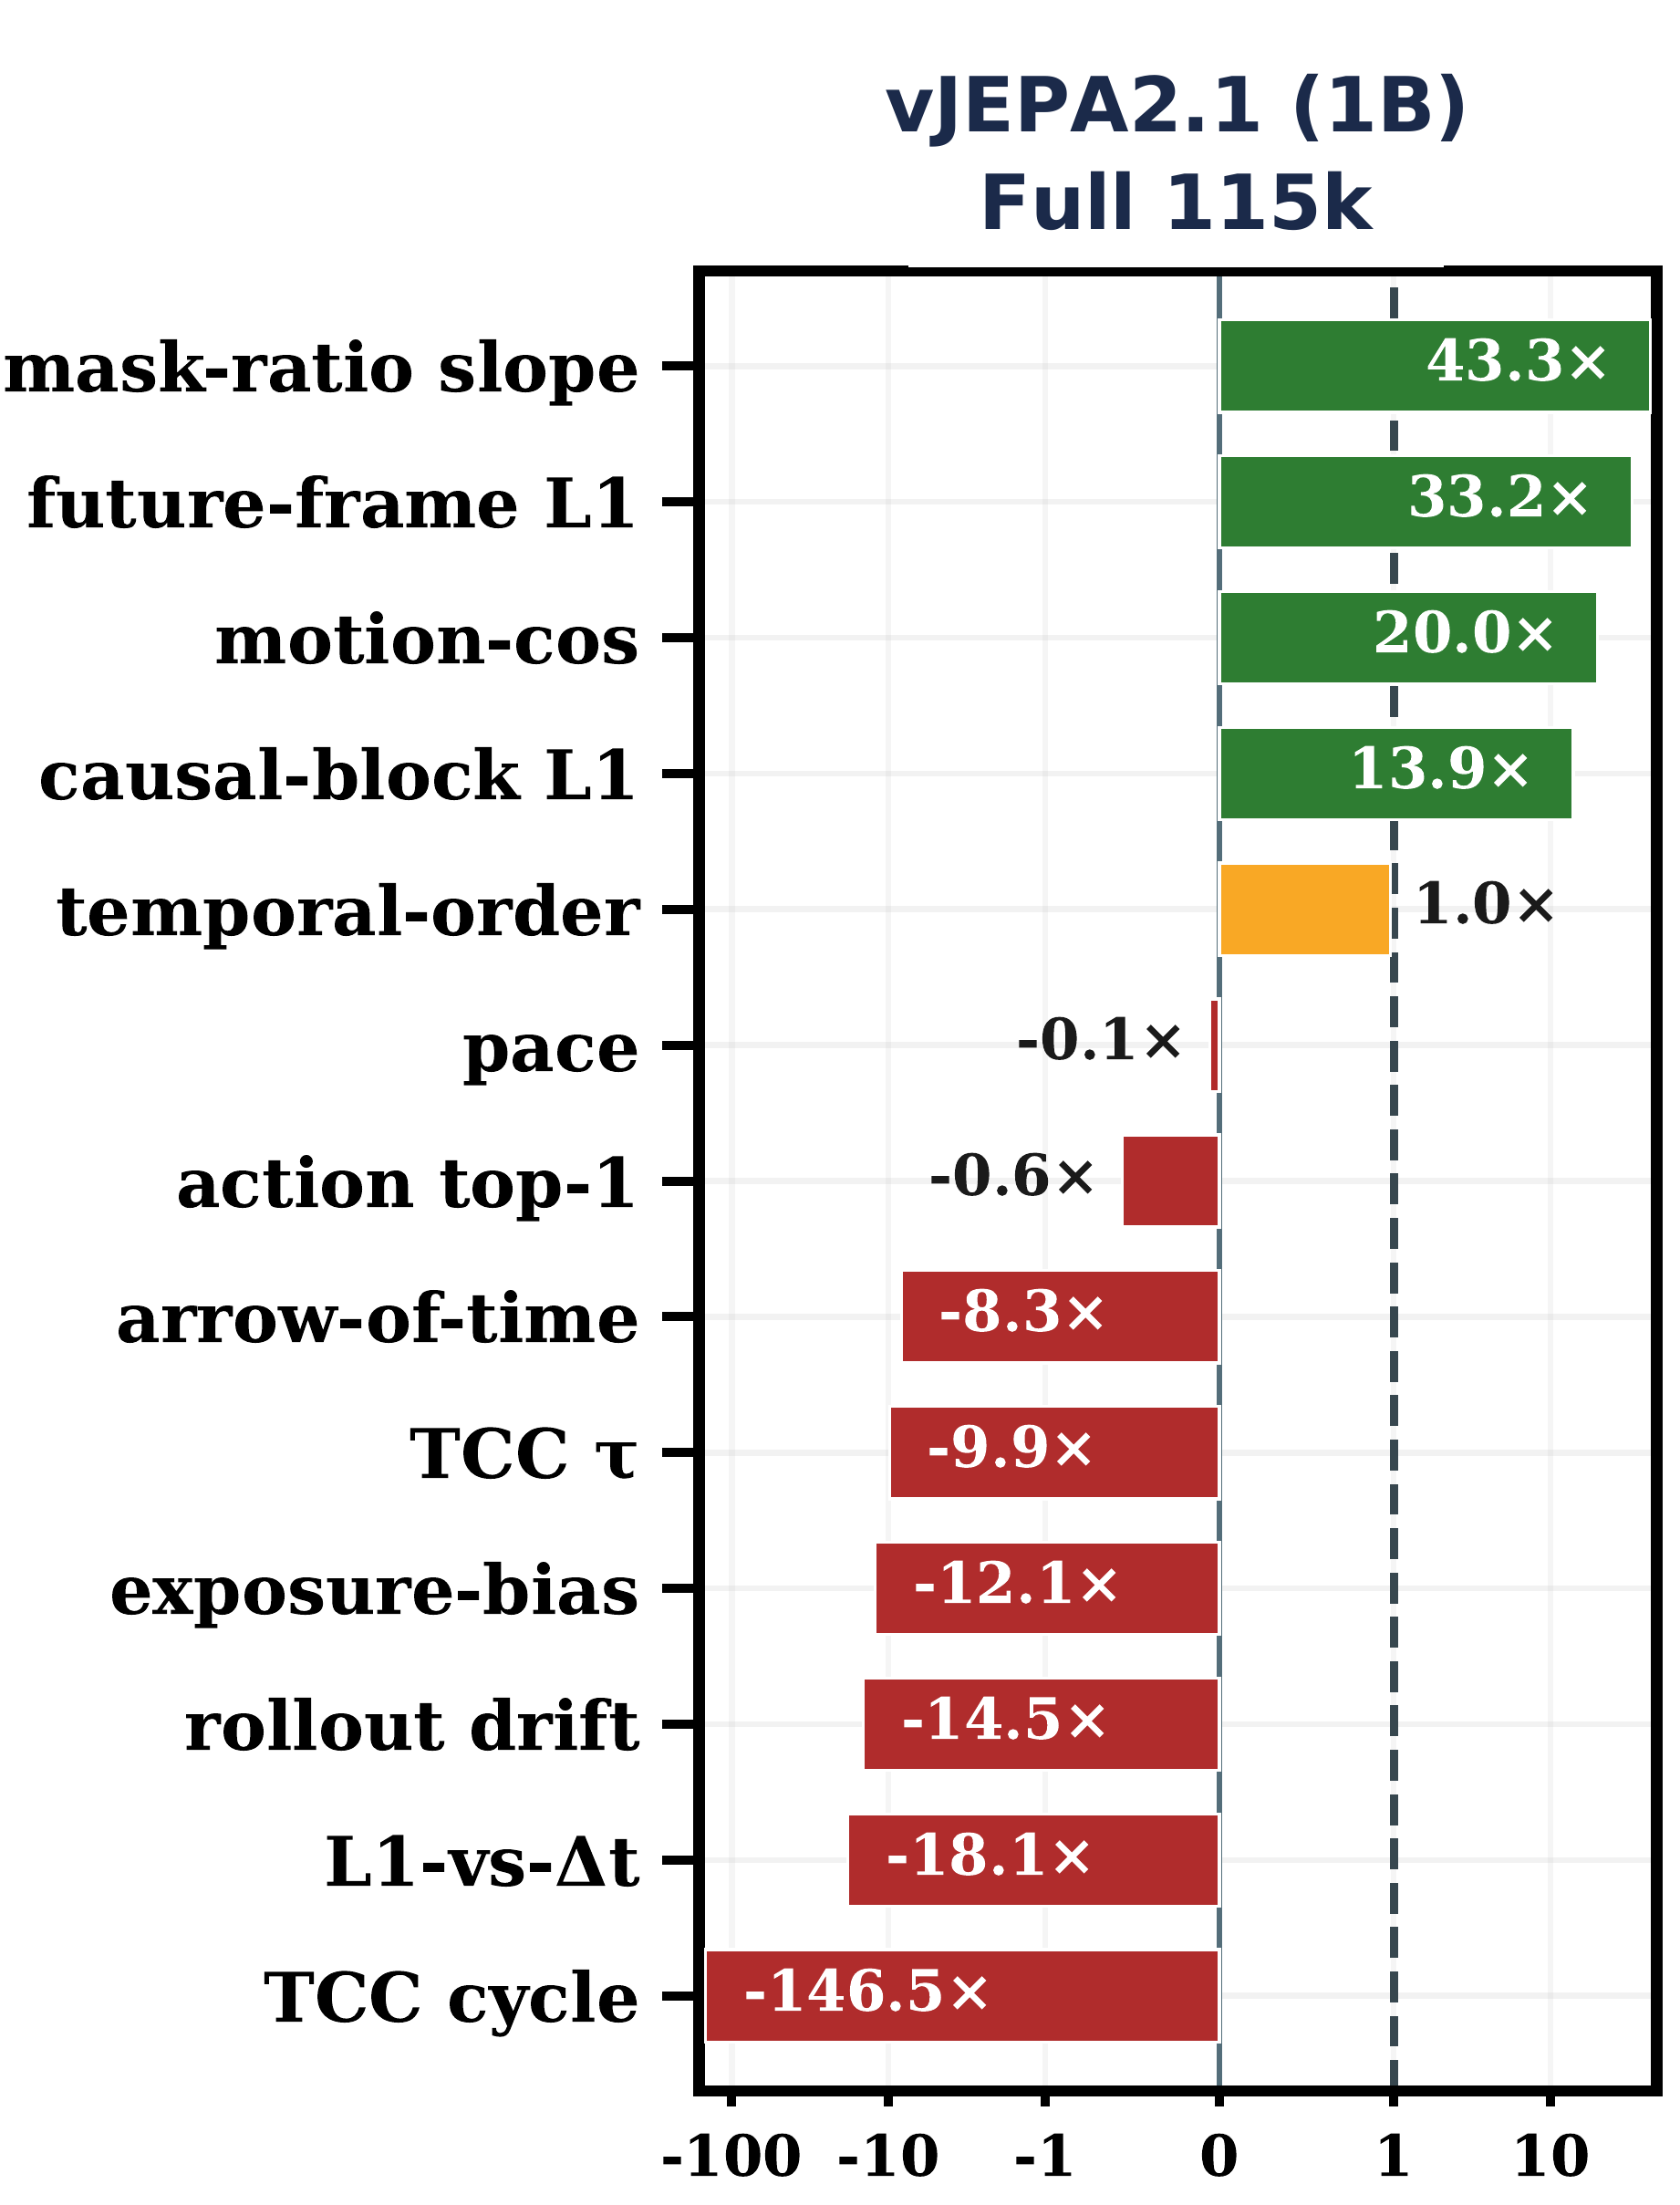
\includegraphics[width=0.97\columnwidth]{figures/forest_115k_col.png}
\caption{Separation of the fixed FactorJEPA model from the strongest rival at 1B on the full corpus, in widths of the paired 95\% BCa interval (symmetric-log axis). Green: FactorJEPA ahead by at least one width; yellow: ahead within the interval; red: the rival ahead.}
\label{fig:forest}
\end{figure}

\paragraph{Findings.}
With limited data (Table~\ref{tab:headline}), FactorJEPA separates from the best rival on Future-frame L1 and Causal L1 at both scales and on Mask-ratio slope at 1B, while Motion cosine favors full fine-tuning. After full 115k-clip training, against the two rivals trained at that scale (LoRA and the frozen backbone), FactorJEPA separates on all four diagnostics, Motion cosine included (Figure~\ref{fig:forest}), by 13.9 (Causal L1) to 43.3 (Mask-ratio slope) interval widths. Whether the motion gap to full fine-tuning closes with more data is untested, because full fine-tuning was not run at 115k. Method rankings on the four diagnostics replicate from the 2B to the 1B backbone (Spearman $\rho \geq 0.895$). Below the rule, however, the best rival stays ahead at 115k on six diagnostics (rollout drift, exposure bias, L1-versus-$\Delta t$ decay, arrow-of-time, and the two TCC measures) by 8.3 to 146.5 interval widths. FactorJEPA predicts crowded scenes better one step ahead; it does not yet keep long predicted futures more coherent.

\section{What This Offers Models of Collective Behaviour}

Agent-based and social-force models write interaction rules by hand and fit their parameters to observed trajectories. A world model with separate agent and interaction channels learns a counterpart of those rules from raw video, so the two can be compared on the same scenes: where the learned interaction channel couples road users that a hand-set rule leaves independent, either the rule or the model is missing something. Our results support this use only partly. One-step prediction and robustness to missing evidence, which matter when road users are occluded, improve consistently; temporal coherence over longer rollouts, which a simulation needs, does not. Because the model needs only monocular public video, with no maps or sensors, it can be trained wherever street footage exists, which is what cross-cultural evaluation of behaviour models needs. DENSEWORLD-115k gives that evaluation a dense, non-Western reference, which we hope behaviour modellers will extend with interaction-level labels.

\section{Limitations}

Every diagnostic lives in the frozen V-JEPA embedding space or a linear probe on it; we report no trajectory forecast and no comparison with a calibrated social-force or agent-based model, and the interaction channel is not yet checked against human judgements of who yields to whom. We do not report the cross-channel leakage between layout, agent, and interaction channels that the factorization is meant to limit, and we do not isolate how much of the gain comes from the factor supervision rather than from retraining the predictor at all. The split is clip-level, so test clips can share a source video with training clips, and no test city is held out. All footage is Indian; other dense-traffic regions are untested. Each configuration was trained once.

{\small
\bibliography{factorjepa}
}

\end{document}
